\subsection{Цель выполнения домашнего задания}\label{blockN.VariantM}
\textbf{Цель выполнения домашнего задания }-- \GoalOfResearch

%-------------------------------------------------
\subsection{Задание}
Рассматривается система, аналогичная задаче $№3$, но в которой возможна организация ремонта ранее вышедших из строя устройств.
Одновременно может ремонтироваться только одно устройство.
Если подлежат ремонту устройства разных типов, приоритет отдаётся тем, которых сломалось больше,
а если их сломалось одинаковое число – тому типу, интенсивность поломок которого выше.
Интенсивность ремонта устройств обоих типов одинакова и равна $\lambda_S = (N_A + N_B - (G \bmod 3)) * (G + (N \bmod 4))$.


Если $N$ – номер зачётной книжки, а $G$ – последняя цифра в номере группы,
то параметры системы определяются следующим образом:
\[
\begin{matrix}
    \lambda_A= G + (N \bmod 3) \\
    \lambda_B= G + (N \bmod 5) \\
    N_A= 2 + (G \bmod 2) \\
    N_B= 2 + (N \bmod 2) \\
    R_A= 4 + (G \bmod 2) \\
    R_B= 5 - (G \bmod 2) \\
    \lambda_S = (N_A + N_B - (G \bmod 3)) * (G + (N \bmod 4))
\end{matrix}
\]

Требуется:
\begin{enumerate}
    \item нарисовать граф состояний системы;
    \item составить матрицу интенсивностей переходов;
    \item записать алгебраические уравнения Колмогорова для установившегося режима работы;
    \item рассчитать предельные вероятности состояний системы;
    \item рассчитать математические ожидания прикладных характеристик системы:
    \begin{itemize}
        \item вероятности отказа системы;
        \item числа готовых к эксплуатации устройств каждого типа;
        \item коэффициента загрузки ремонтной службы.
    \end{itemize}
    \item записать дифференциальные уравнения Колмогорова;
    \item методами численного интегрирования решить полученную систему уравнений, исходя из того, что в начальный момент времени все устройства исправны, а время моделирования выбирается вдвое больше теоретической оценки времени переходного процесса (т.е. того времени, которое необходимо, чтобы эвклидова норма вектора невязки с ранее рассчитанным предельным вектором составляла не более 10\% эвклидовой нормы последнего);
    \item построить графики вероятностей нахождения системы в каждом из возможных состояний с течением времени;
    \item провести имитационное моделирование системы в терминах непрерывных марковских цепей 100 раз, время моделирования выбирается вдвое больше экспериментальной оценки времени переходного процесса (т.е. того времени, которое необходимо, чтобы накопленная доля времени пребывания системы в каждом из состояний отличалась не более чем на 10\% от результатов, полученных при обработке предыдущего переключения цепи), проанализировать статистику времени выхода на установившийся режим работы и рассчитать статистические оценки предельных вероятностей после выхода на установившийся режим;
    \item провести имитационное моделирование системы в терминах дискретно-событийного моделирования (с независимым планированием времени наступления событий для каждого устройства в отдельности) 100 раз, время моделирования выбирается вдвое больше экспериментальной оценки времени переходного процесса (т.е. того времени, которое необходимо, чтобы накопленные средние оценки прикладных характеристик системы отличалась не более чем на 10\% от результатов, полученных при обработке предыдущего события в системе), проанализировать статистику времени выхода на установившийся режим работы и рассчитать статистические оценки для прикладных характеристик системы после выхода на установившийся режим.
\end{enumerate}
%-------------------------------------------------
\newpage
\subsection{Решение}

Рассчитаем начальные данные для выполнения домашнего задания по номеру зачетки $N = 46$ и группы $G = 2$:
\[
\begin{matrix}
    \lambda_A & = G + (N \bmod 3) = 2 + (46 \bmod 3) = & 3 \\
    \lambda_B & = G + (N \bmod 5) = 2 + (46 \bmod 5) = & 3 \\
    N_A & = 2 + (G \bmod 2) = 2 + (2 \bmod 2) = & 2 \\
    N_B & = 2 + (N \bmod 2) = 2 + (46 \bmod 2) = & 2 \\
    R_A & = 4 + (G \bmod 2) = 4 + (2 \bmod 2) = & 4 \\
    R_B & = 5 - (G \bmod 2) = 5 - (2 \bmod 2) = & 5 \\
    \lambda_S & = (N_A + N_B - (G \bmod 3)) * (G + (N \bmod 4)) = & 8
\end{matrix}
\]


    Так как по условию ремонт устройства в случае одинакового количества сломанных устройств A и B производится ремонт устройства
    с большей $\lambda$, однако в предложенном варианте эти $\lambda$ получились равны, сделаем $\lambda_A$ на один больше.
    \[\lambda_A = 4\]


Предположим что $S^{ab}_{cd}$ - состояние системы, где
\begin{itemize}
    \item $a$ - количество работающих устройств типа $A$,
    \item $b$ - количество резервных устройств типа $A$,
    \item $c$ - количество работающих устройств типа $B$,
    \item $d$ - количество резервных устройств типа $B$.
\end{itemize}
На рисунке \ref{graph} изображен граф состояний системы.

Для системы с данными параметрами был получен граф состояний системы, представленный на рисунке \ref{graph}. Верхние и нижние индексы -- пара чисел, первое -- рабочие устройства типа $А$ (верхний) или $В$ (нижний), второе -- остаток в резерве.

\begin{figure}[H]

    \centerline{
        \resizebox{10cm}{!}{
                
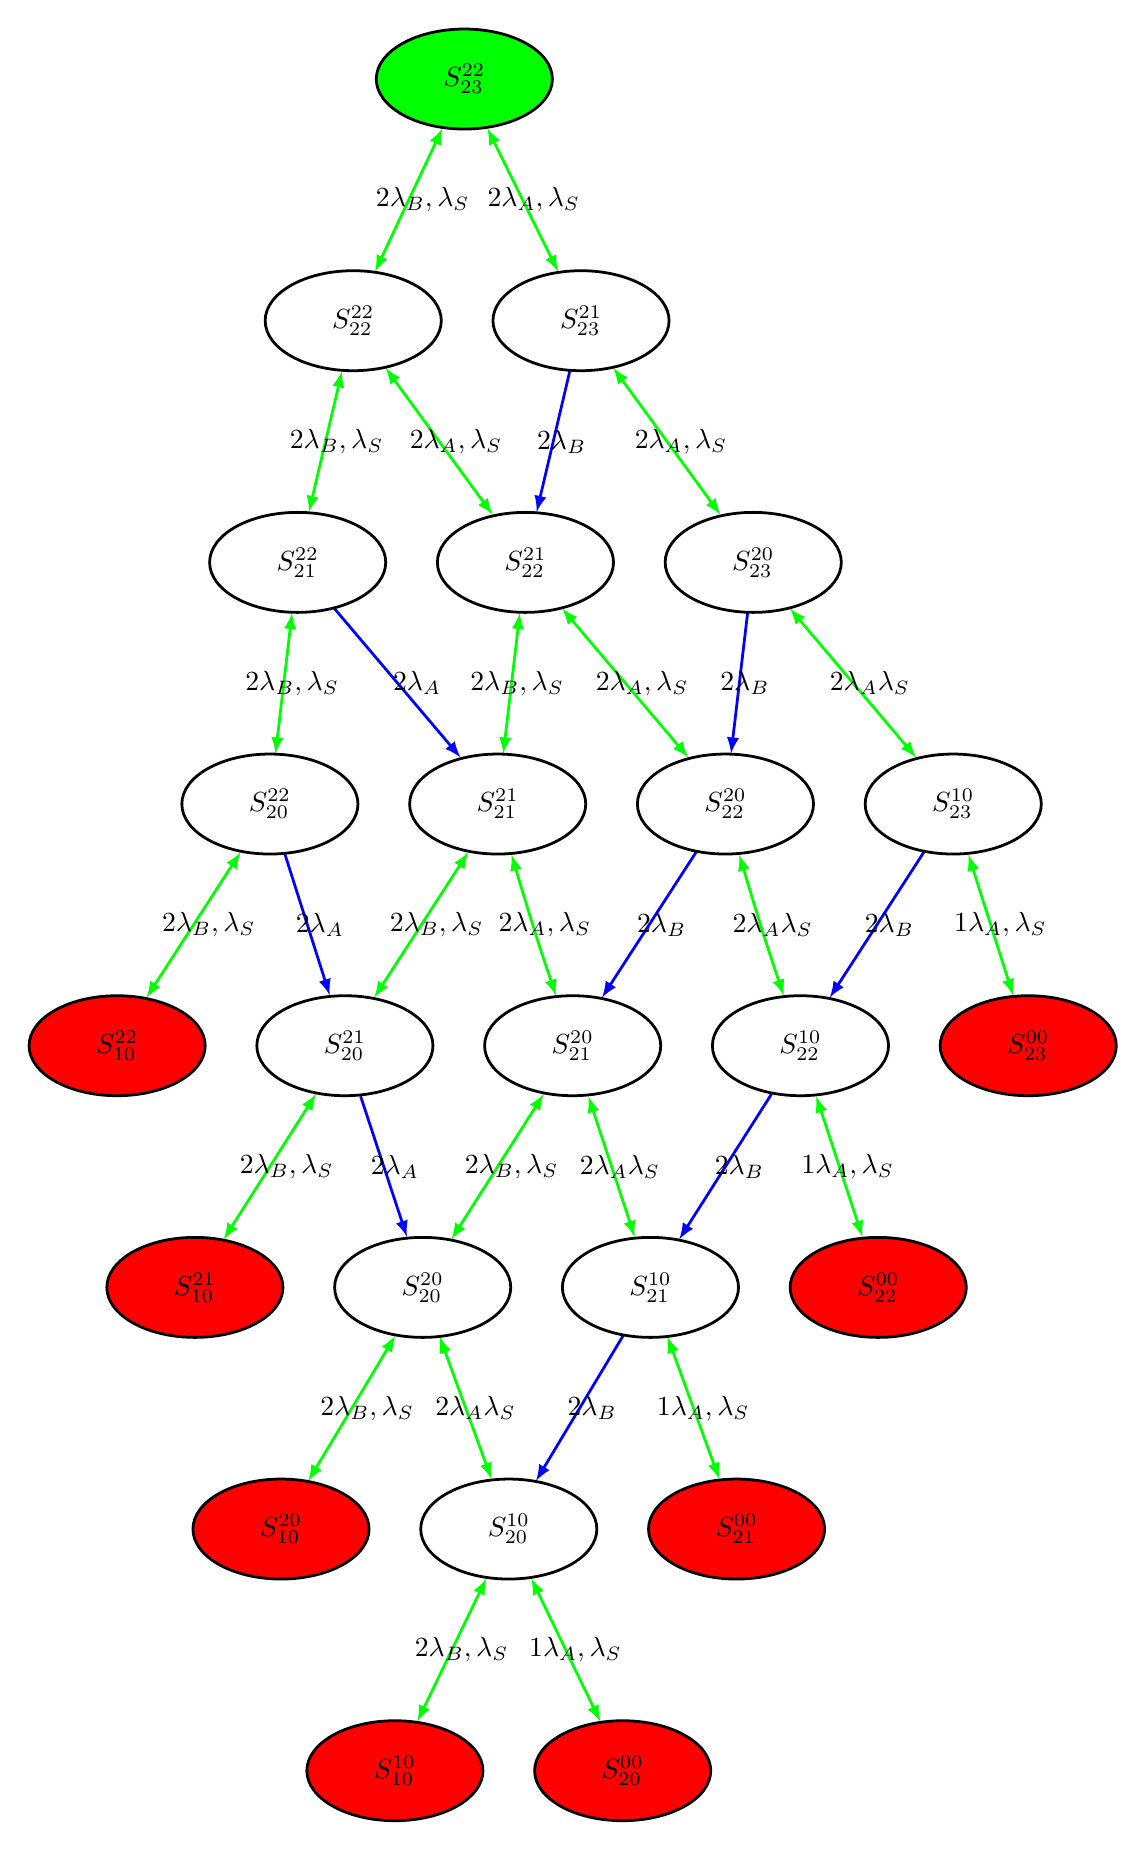
\begin{tikzpicture}[>=latex,line join=bevel,]
  \pgfsetlinewidth{1bp}
%%
\pgfsetcolor{black}
  % Edge: s2223 -> s2222
  \pgfsetcolor{green}
  \draw [<->] (148.94bp,609.21bp) .. controls (139.58bp,589.3bp) and (134.16bp,577.79bp)  .. (124.73bp,557.76bp);
  \definecolor{strokecol}{rgb}{0.0,0.0,0.0};
  \pgfsetstrokecolor{strokecol}
  \draw (141.85bp,583.5bp) node {$2\lambda_B,\lambda_S$};
  % Edge: s2223 -> s2123
  \pgfsetcolor{green}
  \draw [<->] (165.15bp,609.21bp) .. controls (175.04bp,589.19bp) and (180.79bp,577.55bp)  .. (190.57bp,557.76bp);
  \definecolor{strokecol}{rgb}{0.0,0.0,0.0};
  \pgfsetstrokecolor{strokecol}
  \draw (181.85bp,583.5bp) node {$2\lambda_A,\lambda_S$};
  % Edge: s2222 -> s2221
  \pgfsetcolor{green}
  \draw [<->] (112.8bp,521.8bp) .. controls (108.1bp,501.83bp) and (105.6bp,491.19bp)  .. (100.89bp,471.18bp);
  \definecolor{strokecol}{rgb}{0.0,0.0,0.0};
  \pgfsetstrokecolor{strokecol}
  \draw (110.85bp,496.5bp) node {$2\lambda_B,\lambda_S$};
  % Edge: s2222 -> s2122
  \pgfsetcolor{green}
  \draw [<->] (128.51bp,523.01bp) .. controls (142.99bp,503.15bp) and (152.51bp,490.11bp)  .. (167.03bp,470.21bp);
  \definecolor{strokecol}{rgb}{0.0,0.0,0.0};
  \pgfsetstrokecolor{strokecol}
  \draw (153.85bp,496.5bp) node {$2\lambda_A,\lambda_S$};
  % Edge: s2123 -> s2122
  \pgfsetcolor{blue}
  \draw [->] (194.8bp,521.8bp) .. controls (192.09bp,510.28bp) and (188.46bp,494.86bp)  .. (182.89bp,471.18bp);
  \definecolor{strokecol}{rgb}{0.0,0.0,0.0};
  \pgfsetstrokecolor{strokecol}
  \draw (191.85bp,496.5bp) node {$2\lambda_B$};
  % Edge: s2123 -> s2023
  \pgfsetcolor{green}
  \draw [<->] (210.51bp,523.01bp) .. controls (224.99bp,503.15bp) and (234.51bp,490.11bp)  .. (249.03bp,470.21bp);
  \definecolor{strokecol}{rgb}{0.0,0.0,0.0};
  \pgfsetstrokecolor{strokecol}
  \draw (234.85bp,496.5bp) node {$2\lambda_A,\lambda_S$};
  % Edge: s2221 -> s2220
  \pgfsetcolor{green}
  \draw [<->] (94.824bp,434.8bp) .. controls (92.447bp,414.6bp) and (91.224bp,404.2bp)  .. (88.868bp,384.18bp);
  \definecolor{strokecol}{rgb}{0.0,0.0,0.0};
  \pgfsetstrokecolor{strokecol}
  \draw (94.847bp,409.5bp) node {$2\lambda_B,\lambda_S$};
  % Edge: s2221 -> s2121
  \pgfsetcolor{blue}
  \draw [->] (110.05bp,436.41bp) .. controls (120.84bp,423.67bp) and (136.28bp,405.45bp)  .. (155.48bp,382.78bp);
  \definecolor{strokecol}{rgb}{0.0,0.0,0.0};
  \pgfsetstrokecolor{strokecol}
  \draw (139.85bp,409.5bp) node {$2\lambda_A$};
  % Edge: s2122 -> s2121
  \pgfsetcolor{green}
  \draw [<->] (176.82bp,434.8bp) .. controls (174.45bp,414.6bp) and (173.22bp,404.2bp)  .. (170.87bp,384.18bp);
  \definecolor{strokecol}{rgb}{0.0,0.0,0.0};
  \pgfsetstrokecolor{strokecol}
  \draw (175.85bp,409.5bp) node {$2\lambda_B,\lambda_S$};
  % Edge: s2122 -> s2022
  \pgfsetcolor{green}
  \draw [<->] (192.05bp,436.41bp) .. controls (208.7bp,416.76bp) and (220.5bp,402.83bp)  .. (237.48bp,382.78bp);
  \definecolor{strokecol}{rgb}{0.0,0.0,0.0};
  \pgfsetstrokecolor{strokecol}
  \draw (220.85bp,409.5bp) node {$2\lambda_A,\lambda_S$};
  % Edge: s2023 -> s2022
  \pgfsetcolor{blue}
  \draw [->] (258.82bp,434.8bp) .. controls (257.48bp,423.39bp) and (255.69bp,408.16bp)  .. (252.87bp,384.18bp);
  \definecolor{strokecol}{rgb}{0.0,0.0,0.0};
  \pgfsetstrokecolor{strokecol}
  \draw (257.85bp,409.5bp) node {$2\lambda_B$};
  % Edge: s2023 -> s1023
  \pgfsetcolor{green}
  \draw [<->] (274.05bp,436.41bp) .. controls (290.7bp,416.76bp) and (302.5bp,402.83bp)  .. (319.48bp,382.78bp);
  \definecolor{strokecol}{rgb}{0.0,0.0,0.0};
  \pgfsetstrokecolor{strokecol}
  \draw (302.85bp,409.5bp) node {$2\lambda_A\lambda_S$};
  % Edge: s2220 -> s2210
  \pgfsetcolor{green}
  \draw [<->] (76.243bp,348.61bp) .. controls (63.334bp,328.66bp) and (55.192bp,316.08bp)  .. (42.419bp,296.34bp);
  \definecolor{strokecol}{rgb}{0.0,0.0,0.0};
  \pgfsetstrokecolor{strokecol}
  \draw (64.847bp,322.5bp) node {$2\lambda_B,\lambda_S$};
  % Edge: s2220 -> s2120
  \pgfsetcolor{blue}
  \draw [->] (92.311bp,347.8bp) .. controls (95.971bp,336.28bp) and (100.87bp,320.86bp)  .. (108.39bp,297.18bp);
  \definecolor{strokecol}{rgb}{0.0,0.0,0.0};
  \pgfsetstrokecolor{strokecol}
  \draw (104.85bp,322.5bp) node {$2\lambda_A$};
  % Edge: s2121 -> s2120
  \pgfsetcolor{green}
  \draw [<->] (158.24bp,348.61bp) .. controls (145.33bp,328.66bp) and (137.19bp,316.08bp)  .. (124.42bp,296.34bp);
  \definecolor{strokecol}{rgb}{0.0,0.0,0.0};
  \pgfsetstrokecolor{strokecol}
  \draw (146.85bp,322.5bp) node {$2\lambda_B,\lambda_S$};
  % Edge: s2121 -> s2021
  \pgfsetcolor{green}
  \draw [<->] (173.82bp,347.82bp) .. controls (179.12bp,330.06bp) and (181.53bp,322.22bp)  .. (183.85bp,315.0bp) .. controls (184.64bp,312.52bp) and (185.49bp,309.95bp)  .. (189.85bp,297.05bp);
  \definecolor{strokecol}{rgb}{0.0,0.0,0.0};
  \pgfsetstrokecolor{strokecol}
  \draw (185.85bp,322.5bp) node {$2\lambda_A,\lambda_S$};
  % Edge: s2022 -> s2021
  \pgfsetcolor{blue}
  \draw [->] (240.24bp,348.61bp) .. controls (232.33bp,336.38bp) and (221.37bp,319.44bp)  .. (206.42bp,296.34bp);
  \definecolor{strokecol}{rgb}{0.0,0.0,0.0};
  \pgfsetstrokecolor{strokecol}
  \draw (227.85bp,322.5bp) node {$2\lambda_B$};
  % Edge: s2022 -> s1022
  \pgfsetcolor{green}
  \draw [<->] (255.82bp,347.82bp) .. controls (261.12bp,330.06bp) and (263.53bp,322.22bp)  .. (265.85bp,315.0bp) .. controls (266.64bp,312.52bp) and (267.49bp,309.95bp)  .. (271.85bp,297.05bp);
  \definecolor{strokecol}{rgb}{0.0,0.0,0.0};
  \pgfsetstrokecolor{strokecol}
  \draw (267.85bp,322.5bp) node {$2\lambda_A\lambda_S$};
  % Edge: s1023 -> s1022
  \pgfsetcolor{blue}
  \draw [->] (322.24bp,348.61bp) .. controls (314.33bp,336.38bp) and (303.37bp,319.44bp)  .. (288.42bp,296.34bp);
  \definecolor{strokecol}{rgb}{0.0,0.0,0.0};
  \pgfsetstrokecolor{strokecol}
  \draw (309.85bp,322.5bp) node {$2\lambda_B$};
  % Edge: s1023 -> s0023
  \pgfsetcolor{green}
  \draw [<->] (338.31bp,347.8bp) .. controls (344.69bp,327.73bp) and (348.11bp,316.96bp)  .. (354.39bp,297.18bp);
  \definecolor{strokecol}{rgb}{0.0,0.0,0.0};
  \pgfsetstrokecolor{strokecol}
  \draw (349.85bp,322.5bp) node {$1\lambda_A,\lambda_S$};
  % Edge: s2120 -> s2110
  \pgfsetcolor{green}
  \draw [<->] (103.44bp,261.61bp) .. controls (90.831bp,241.77bp) and (82.929bp,229.33bp)  .. (70.227bp,209.34bp);
  \definecolor{strokecol}{rgb}{0.0,0.0,0.0};
  \pgfsetstrokecolor{strokecol}
  \draw (92.847bp,235.5bp) node {$2\lambda_B,\lambda_S$};
  % Edge: s2120 -> s2020
  \pgfsetcolor{blue}
  \draw [->] (119.51bp,260.8bp) .. controls (123.35bp,249.16bp) and (128.49bp,233.55bp)  .. (136.19bp,210.18bp);
  \definecolor{strokecol}{rgb}{0.0,0.0,0.0};
  \pgfsetstrokecolor{strokecol}
  \draw (131.85bp,235.5bp) node {$2\lambda_A$};
  % Edge: s2021 -> s2020
  \pgfsetcolor{green}
  \draw [<->] (185.44bp,261.61bp) .. controls (172.83bp,241.77bp) and (164.93bp,229.33bp)  .. (152.23bp,209.34bp);
  \definecolor{strokecol}{rgb}{0.0,0.0,0.0};
  \pgfsetstrokecolor{strokecol}
  \draw (173.85bp,235.5bp) node {$2\lambda_B,\lambda_S$};
  % Edge: s2021 -> s1021
  \pgfsetcolor{green}
  \draw [<->] (201.51bp,260.8bp) .. controls (208.02bp,241.06bp) and (211.6bp,230.17bp)  .. (218.19bp,210.18bp);
  \definecolor{strokecol}{rgb}{0.0,0.0,0.0};
  \pgfsetstrokecolor{strokecol}
  \draw (212.85bp,235.5bp) node {$2\lambda_A\lambda_S$};
  % Edge: s1022 -> s1021
  \pgfsetcolor{blue}
  \draw [->] (267.44bp,261.61bp) .. controls (259.67bp,249.38bp) and (248.91bp,232.44bp)  .. (234.23bp,209.34bp);
  \definecolor{strokecol}{rgb}{0.0,0.0,0.0};
  \pgfsetstrokecolor{strokecol}
  \draw (255.85bp,235.5bp) node {$2\lambda_B$};
  % Edge: s1022 -> s0022
  \pgfsetcolor{green}
  \draw [<->] (283.51bp,260.8bp) .. controls (290.02bp,241.06bp) and (293.6bp,230.17bp)  .. (300.19bp,210.18bp);
  \definecolor{strokecol}{rgb}{0.0,0.0,0.0};
  \pgfsetstrokecolor{strokecol}
  \draw (294.85bp,235.5bp) node {$1\lambda_A,\lambda_S$};
  % Edge: s2020 -> s2010
  \pgfsetcolor{green}
  \draw [<->] (132.01bp,174.61bp) .. controls (120.11bp,154.77bp) and (112.65bp,142.33bp)  .. (100.65bp,122.34bp);
  \definecolor{strokecol}{rgb}{0.0,0.0,0.0};
  \pgfsetstrokecolor{strokecol}
  \draw (121.85bp,148.5bp) node {$2\lambda_B,\lambda_S$};
  % Edge: s2020 -> s1020
  \pgfsetcolor{green}
  \draw [<->] (147.97bp,174.21bp) .. controls (155.27bp,154.21bp) and (159.34bp,143.04bp)  .. (166.63bp,123.05bp);
  \definecolor{strokecol}{rgb}{0.0,0.0,0.0};
  \pgfsetstrokecolor{strokecol}
  \draw (160.85bp,148.5bp) node {$2\lambda_A\lambda_S$};
  % Edge: s1021 -> s1020
  \pgfsetcolor{blue}
  \draw [->] (214.01bp,174.61bp) .. controls (206.68bp,162.38bp) and (196.51bp,145.44bp)  .. (182.65bp,122.34bp);
  \definecolor{strokecol}{rgb}{0.0,0.0,0.0};
  \pgfsetstrokecolor{strokecol}
  \draw (202.85bp,148.5bp) node {$2\lambda_B$};
  % Edge: s1021 -> s0021
  \pgfsetcolor{green}
  \draw [<->] (229.97bp,174.21bp) .. controls (237.27bp,154.21bp) and (241.34bp,143.04bp)  .. (248.63bp,123.05bp);
  \definecolor{strokecol}{rgb}{0.0,0.0,0.0};
  \pgfsetstrokecolor{strokecol}
  \draw (242.85bp,148.5bp) node {$1\lambda_A,\lambda_S$};
  % Edge: s1020 -> s1010
  \pgfsetcolor{green}
  \draw [<->] (164.75bp,87.207bp) .. controls (155.09bp,67.191bp) and (149.48bp,55.547bp)  .. (139.93bp,35.758bp);
  \definecolor{strokecol}{rgb}{0.0,0.0,0.0};
  \pgfsetstrokecolor{strokecol}
  \draw (155.85bp,61.5bp) node {$2\lambda_B,\lambda_S$};
  % Edge: s1020 -> s0020
  \pgfsetcolor{green}
  \draw [<->] (180.95bp,87.207bp) .. controls (190.6bp,67.191bp) and (196.22bp,55.547bp)  .. (205.76bp,35.758bp);
  \definecolor{strokecol}{rgb}{0.0,0.0,0.0};
  \pgfsetstrokecolor{strokecol}
  \draw (196.85bp,61.5bp) node {$1\lambda_A,\lambda_S$};
  % Node: s2223
\begin{scope}
  \definecolor{strokecol}{rgb}{0.0,0.0,0.0};
  \pgfsetstrokecolor{strokecol}
  \definecolor{fillcol}{rgb}{0.0,1.0,0.0};
  \pgfsetfillcolor{fillcol}
  \filldraw [opacity=1] (156.85bp,627.0bp) ellipse (31.7bp and 18.0bp);
  \draw (156.85bp,627.0bp) node {$S^{22}_{23}$};
\end{scope}
  % Node: s2222
\begin{scope}
  \definecolor{strokecol}{rgb}{0.0,0.0,0.0};
  \pgfsetstrokecolor{strokecol}
  \draw (116.85bp,540.0bp) ellipse (31.7bp and 18.0bp);
  \draw (116.85bp,540.0bp) node {$S^{22}_{22}$};
\end{scope}
  % Node: s2123
\begin{scope}
  \definecolor{strokecol}{rgb}{0.0,0.0,0.0};
  \pgfsetstrokecolor{strokecol}
  \draw (198.85bp,540.0bp) ellipse (31.7bp and 18.0bp);
  \draw (198.85bp,540.0bp) node {$S^{21}_{23}$};
\end{scope}
  % Node: s2221
\begin{scope}
  \definecolor{strokecol}{rgb}{0.0,0.0,0.0};
  \pgfsetstrokecolor{strokecol}
  \draw (96.85bp,453.0bp) ellipse (31.7bp and 18.0bp);
  \draw (96.847bp,453.0bp) node {$S^{22}_{21}$};
\end{scope}
  % Node: s2122
\begin{scope}
  \definecolor{strokecol}{rgb}{0.0,0.0,0.0};
  \pgfsetstrokecolor{strokecol}
  \draw (178.85bp,453.0bp) ellipse (31.7bp and 18.0bp);
  \draw (178.85bp,453.0bp) node {$S^{21}_{22}$};
\end{scope}
  % Node: s2023
\begin{scope}
  \definecolor{strokecol}{rgb}{0.0,0.0,0.0};
  \pgfsetstrokecolor{strokecol}
  \draw (260.85bp,453.0bp) ellipse (31.7bp and 18.0bp);
  \draw (260.85bp,453.0bp) node {$S^{20}_{23}$};
\end{scope}
  % Node: s2220
\begin{scope}
  \definecolor{strokecol}{rgb}{0.0,0.0,0.0};
  \pgfsetstrokecolor{strokecol}
  \draw (86.85bp,366.0bp) ellipse (31.7bp and 18.0bp);
  \draw (86.847bp,366.0bp) node {$S^{22}_{20}$};
\end{scope}
  % Node: s2121
\begin{scope}
  \definecolor{strokecol}{rgb}{0.0,0.0,0.0};
  \pgfsetstrokecolor{strokecol}
  \draw (168.85bp,366.0bp) ellipse (31.7bp and 18.0bp);
  \draw (168.85bp,366.0bp) node {$S^{21}_{21}$};
\end{scope}
  % Node: s2022
\begin{scope}
  \definecolor{strokecol}{rgb}{0.0,0.0,0.0};
  \pgfsetstrokecolor{strokecol}
  \draw (250.85bp,366.0bp) ellipse (31.7bp and 18.0bp);
  \draw (250.85bp,366.0bp) node {$S^{20}_{22}$};
\end{scope}
  % Node: s1023
\begin{scope}
  \definecolor{strokecol}{rgb}{0.0,0.0,0.0};
  \pgfsetstrokecolor{strokecol}
  \draw (332.85bp,366.0bp) ellipse (31.7bp and 18.0bp);
  \draw (332.85bp,366.0bp) node {$S^{10}_{23}$};
\end{scope}
  % Node: s2210
\begin{scope}
  \definecolor{strokecol}{rgb}{0.0,0.0,0.0};
  \pgfsetstrokecolor{strokecol}
  \definecolor{fillcol}{rgb}{1.0,0.0,0.0};
  \pgfsetfillcolor{fillcol}
  \filldraw [opacity=1] (31.85bp,279.0bp) ellipse (31.7bp and 18.0bp);
  \draw (31.847bp,279.0bp) node {$S^{22}_{10}$};
\end{scope}
  % Node: s2120
\begin{scope}
  \definecolor{strokecol}{rgb}{0.0,0.0,0.0};
  \pgfsetstrokecolor{strokecol}
  \draw (113.85bp,279.0bp) ellipse (31.7bp and 18.0bp);
  \draw (113.85bp,279.0bp) node {$S^{21}_{20}$};
\end{scope}
  % Node: s2021
\begin{scope}
  \definecolor{strokecol}{rgb}{0.0,0.0,0.0};
  \pgfsetstrokecolor{strokecol}
  \draw (195.85bp,279.0bp) ellipse (31.7bp and 18.0bp);
  \draw (195.85bp,279.0bp) node {$S^{20}_{21}$};
\end{scope}
  % Node: s1022
\begin{scope}
  \definecolor{strokecol}{rgb}{0.0,0.0,0.0};
  \pgfsetstrokecolor{strokecol}
  \draw (277.85bp,279.0bp) ellipse (31.7bp and 18.0bp);
  \draw (277.85bp,279.0bp) node {$S^{10}_{22}$};
\end{scope}
  % Node: s0023
\begin{scope}
  \definecolor{strokecol}{rgb}{0.0,0.0,0.0};
  \pgfsetstrokecolor{strokecol}
  \definecolor{fillcol}{rgb}{1.0,0.0,0.0};
  \pgfsetfillcolor{fillcol}
  \filldraw [opacity=1] (359.85bp,279.0bp) ellipse (31.7bp and 18.0bp);
  \draw (359.85bp,279.0bp) node {$S^{00}_{23}$};
\end{scope}
  % Node: s2110
\begin{scope}
  \definecolor{strokecol}{rgb}{0.0,0.0,0.0};
  \pgfsetstrokecolor{strokecol}
  \definecolor{fillcol}{rgb}{1.0,0.0,0.0};
  \pgfsetfillcolor{fillcol}
  \filldraw [opacity=1] (59.85bp,192.0bp) ellipse (31.7bp and 18.0bp);
  \draw (59.847bp,192.0bp) node {$S^{21}_{10}$};
\end{scope}
  % Node: s2020
\begin{scope}
  \definecolor{strokecol}{rgb}{0.0,0.0,0.0};
  \pgfsetstrokecolor{strokecol}
  \draw (141.85bp,192.0bp) ellipse (31.7bp and 18.0bp);
  \draw (141.85bp,192.0bp) node {$S^{20}_{20}$};
\end{scope}
  % Node: s1021
\begin{scope}
  \definecolor{strokecol}{rgb}{0.0,0.0,0.0};
  \pgfsetstrokecolor{strokecol}
  \draw (223.85bp,192.0bp) ellipse (31.7bp and 18.0bp);
  \draw (223.85bp,192.0bp) node {$S^{10}_{21}$};
\end{scope}
  % Node: s0022
\begin{scope}
  \definecolor{strokecol}{rgb}{0.0,0.0,0.0};
  \pgfsetstrokecolor{strokecol}
  \definecolor{fillcol}{rgb}{1.0,0.0,0.0};
  \pgfsetfillcolor{fillcol}
  \filldraw [opacity=1] (305.85bp,192.0bp) ellipse (31.7bp and 18.0bp);
  \draw (305.85bp,192.0bp) node {$S^{00}_{22}$};
\end{scope}
  % Node: s2010
\begin{scope}
  \definecolor{strokecol}{rgb}{0.0,0.0,0.0};
  \pgfsetstrokecolor{strokecol}
  \definecolor{fillcol}{rgb}{1.0,0.0,0.0};
  \pgfsetfillcolor{fillcol}
  \filldraw [opacity=1] (90.85bp,105.0bp) ellipse (31.7bp and 18.0bp);
  \draw (90.847bp,105.0bp) node {$S^{20}_{10}$};
\end{scope}
  % Node: s1020
\begin{scope}
  \definecolor{strokecol}{rgb}{0.0,0.0,0.0};
  \pgfsetstrokecolor{strokecol}
  \draw (172.85bp,105.0bp) ellipse (31.7bp and 18.0bp);
  \draw (172.85bp,105.0bp) node {$S^{10}_{20}$};
\end{scope}
  % Node: s0021
\begin{scope}
  \definecolor{strokecol}{rgb}{0.0,0.0,0.0};
  \pgfsetstrokecolor{strokecol}
  \definecolor{fillcol}{rgb}{1.0,0.0,0.0};
  \pgfsetfillcolor{fillcol}
  \filldraw [opacity=1] (254.85bp,105.0bp) ellipse (31.7bp and 18.0bp);
  \draw (254.85bp,105.0bp) node {$S^{00}_{21}$};
\end{scope}
  % Node: s1010
\begin{scope}
  \definecolor{strokecol}{rgb}{0.0,0.0,0.0};
  \pgfsetstrokecolor{strokecol}
  \definecolor{fillcol}{rgb}{1.0,0.0,0.0};
  \pgfsetfillcolor{fillcol}
  \filldraw [opacity=1] (131.85bp,18.0bp) ellipse (31.7bp and 18.0bp);
  \draw (131.85bp,18.0bp) node {$S^{10}_{10}$};
\end{scope}
  % Node: s0020
\begin{scope}
  \definecolor{strokecol}{rgb}{0.0,0.0,0.0};
  \pgfsetstrokecolor{strokecol}
  \definecolor{fillcol}{rgb}{1.0,0.0,0.0};
  \pgfsetfillcolor{fillcol}
  \filldraw [opacity=1] (213.85bp,18.0bp) ellipse (31.7bp and 18.0bp);
  \draw (213.85bp,18.0bp) node {$S^{00}_{20}$};
\end{scope}
%
\end{tikzpicture}

        }
%        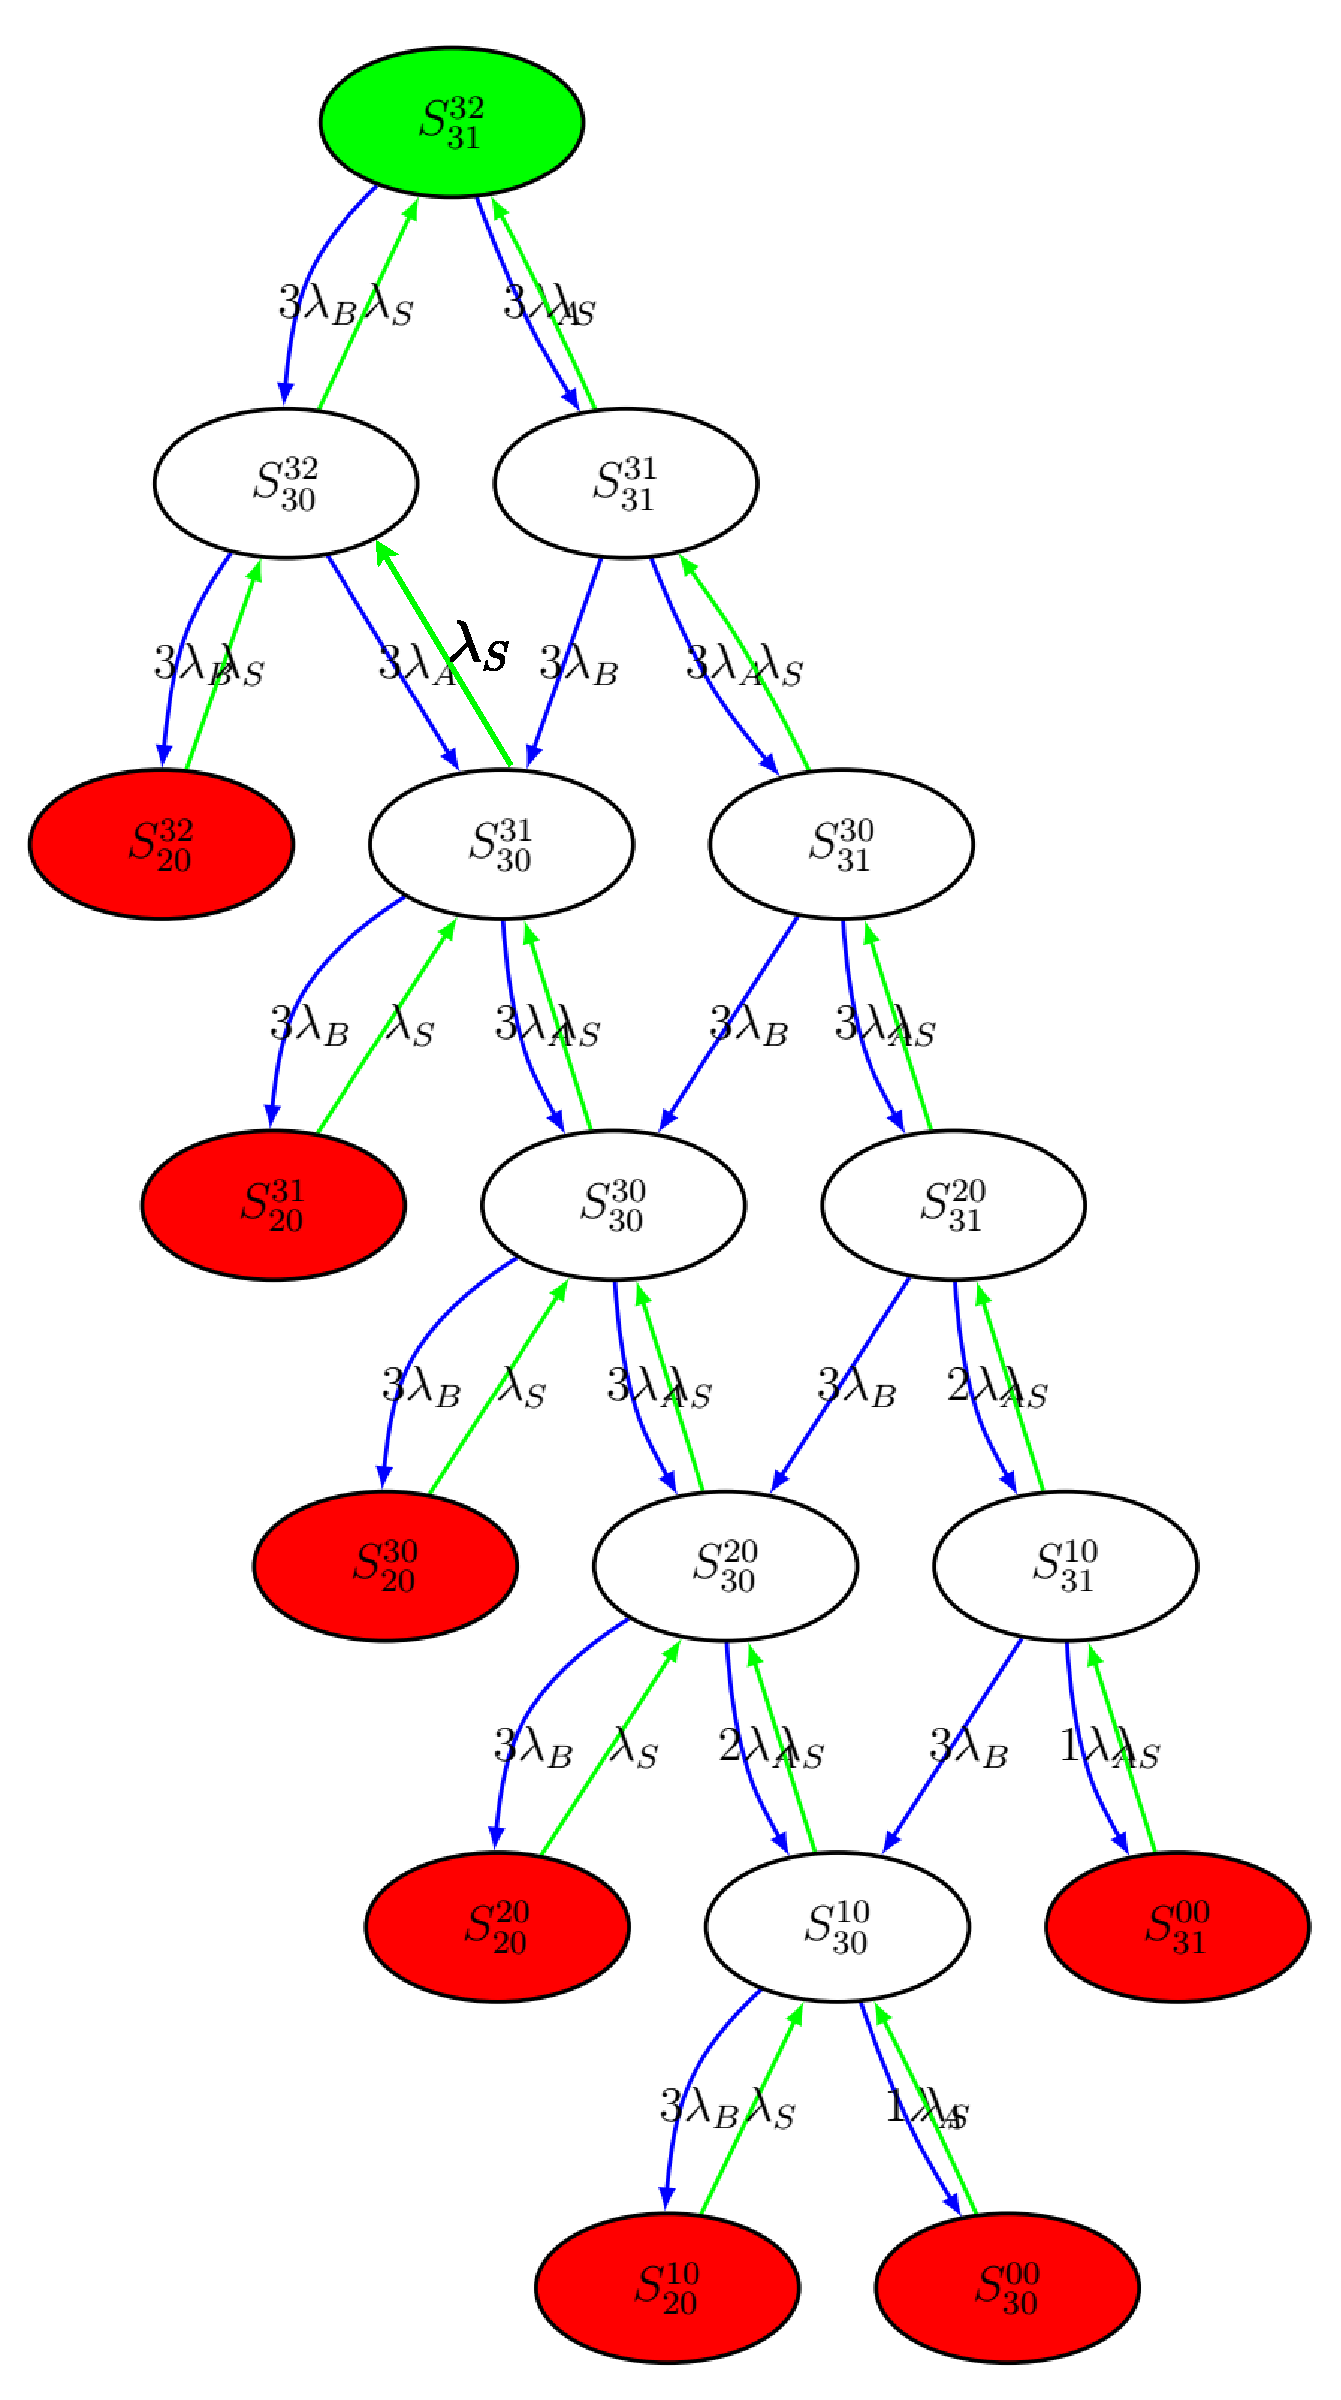
\includegraphics[height=0.8\textheight]{Images/graph.pdf}
    }

    \caption{Граф состояний системы ($\lambda_A = 4$, $\lambda_B = 3$)}
    \label{graph}
\end{figure}

\newpage
По данному графу была получена матрица интенсивности:

\[
    \resizebox{\textwidth}{!}{$
        \Lambda =
        \begin{pmatrix}
        -14 & 6 & 8 & 0 & 0 & 0 & 0 & 0 & 0 & 0 & 0 & 0 & 0 & 0 & 0 & 0 & 0 & 0 & 0 & 0 & 0 & 0 & 0 & 0 \\
8 & -22 & 0 & 6 & 8 & 0 & 0 & 0 & 0 & 0 & 0 & 0 & 0 & 0 & 0 & 0 & 0 & 0 & 0 & 0 & 0 & 0 & 0 & 0 \\
8 & 0 & -22 & 0 & 6 & 8 & 0 & 0 & 0 & 0 & 0 & 0 & 0 & 0 & 0 & 0 & 0 & 0 & 0 & 0 & 0 & 0 & 0 & 0 \\
0 & 8 & 0 & -22 & 0 & 0 & 6 & 8 & 0 & 0 & 0 & 0 & 0 & 0 & 0 & 0 & 0 & 0 & 0 & 0 & 0 & 0 & 0 & 0 \\
0 & 8 & 0 & 0 & -22 & 0 & 0 & 6 & 8 & 0 & 0 & 0 & 0 & 0 & 0 & 0 & 0 & 0 & 0 & 0 & 0 & 0 & 0 & 0 \\
0 & 0 & 8 & 0 & 0 & -22 & 0 & 0 & 6 & 8 & 0 & 0 & 0 & 0 & 0 & 0 & 0 & 0 & 0 & 0 & 0 & 0 & 0 & 0 \\
0 & 0 & 0 & 8 & 0 & 0 & -22 & 0 & 0 & 0 & 6 & 8 & 0 & 0 & 0 & 0 & 0 & 0 & 0 & 0 & 0 & 0 & 0 & 0 \\
0 & 0 & 0 & 0 & 8 & 0 & 0 & -22 & 0 & 0 & 0 & 6 & 8 & 0 & 0 & 0 & 0 & 0 & 0 & 0 & 0 & 0 & 0 & 0 \\
0 & 0 & 0 & 0 & 8 & 0 & 0 & 0 & -22 & 0 & 0 & 0 & 6 & 8 & 0 & 0 & 0 & 0 & 0 & 0 & 0 & 0 & 0 & 0 \\
0 & 0 & 0 & 0 & 0 & 8 & 0 & 0 & 0 & -18 & 0 & 0 & 0 & 6 & 4 & 0 & 0 & 0 & 0 & 0 & 0 & 0 & 0 & 0 \\
0 & 0 & 0 & 0 & 0 & 0 & 8 & 0 & 0 & 0 & -8 & 0 & 0 & 0 & 0 & 0 & 0 & 0 & 0 & 0 & 0 & 0 & 0 & 0 \\
0 & 0 & 0 & 0 & 0 & 0 & 0 & 8 & 0 & 0 & 0 & -22 & 0 & 0 & 0 & 6 & 8 & 0 & 0 & 0 & 0 & 0 & 0 & 0 \\
0 & 0 & 0 & 0 & 0 & 0 & 0 & 8 & 0 & 0 & 0 & 0 & -22 & 0 & 0 & 0 & 6 & 8 & 0 & 0 & 0 & 0 & 0 & 0 \\
0 & 0 & 0 & 0 & 0 & 0 & 0 & 0 & 8 & 0 & 0 & 0 & 0 & -18 & 0 & 0 & 0 & 6 & 4 & 0 & 0 & 0 & 0 & 0 \\
0 & 0 & 0 & 0 & 0 & 0 & 0 & 0 & 0 & 8 & 0 & 0 & 0 & 0 & -8 & 0 & 0 & 0 & 0 & 0 & 0 & 0 & 0 & 0 \\
0 & 0 & 0 & 0 & 0 & 0 & 0 & 0 & 0 & 0 & 0 & 8 & 0 & 0 & 0 & -8 & 0 & 0 & 0 & 0 & 0 & 0 & 0 & 0 \\
0 & 0 & 0 & 0 & 0 & 0 & 0 & 0 & 0 & 0 & 0 & 0 & 8 & 0 & 0 & 0 & -22 & 0 & 0 & 6 & 8 & 0 & 0 & 0 \\
0 & 0 & 0 & 0 & 0 & 0 & 0 & 0 & 0 & 0 & 0 & 0 & 8 & 0 & 0 & 0 & 0 & -18 & 0 & 0 & 6 & 4 & 0 & 0 \\
0 & 0 & 0 & 0 & 0 & 0 & 0 & 0 & 0 & 0 & 0 & 0 & 0 & 8 & 0 & 0 & 0 & 0 & -8 & 0 & 0 & 0 & 0 & 0 \\
0 & 0 & 0 & 0 & 0 & 0 & 0 & 0 & 0 & 0 & 0 & 0 & 0 & 0 & 0 & 0 & 8 & 0 & 0 & -8 & 0 & 0 & 0 & 0 \\
0 & 0 & 0 & 0 & 0 & 0 & 0 & 0 & 0 & 0 & 0 & 0 & 0 & 0 & 0 & 0 & 8 & 0 & 0 & 0 & -18 & 0 & 6 & 4 \\
0 & 0 & 0 & 0 & 0 & 0 & 0 & 0 & 0 & 0 & 0 & 0 & 0 & 0 & 0 & 0 & 0 & 8 & 0 & 0 & 0 & -8 & 0 & 0 \\
0 & 0 & 0 & 0 & 0 & 0 & 0 & 0 & 0 & 0 & 0 & 0 & 0 & 0 & 0 & 0 & 0 & 0 & 0 & 0 & 8 & 0 & -8 & 0 \\
0 & 0 & 0 & 0 & 0 & 0 & 0 & 0 & 0 & 0 & 0 & 0 & 0 & 0 & 0 & 0 & 0 & 0 & 0 & 0 & 8 & 0 & 0 & -8 
        \end{pmatrix}
    $}
\]

\subsection{Уравнения Колмогорова}
Составим систему алгебраических уравнений Колмогорова для установившегося режима работы.

\[
\begin{cases}
    0 =-14p_{0} +8p_{1} +8p_{2} \\ 
0 = 6p_{0} -22p_{1} +8p_{3} +8p_{4} \\ 
0 = 8p_{0} -22p_{2} +8p_{5} \\ 
0 = 6p_{1} -22p_{3} +8p_{6} \\ 
0 = 8p_{1} +6p_{2} -22p_{4} +8p_{7} +8p_{8} \\ 
0 = 8p_{2} -22p_{5} +8p_{9} \\ 
0 = 6p_{3} -22p_{6} +8p_{10} \\ 
0 = 8p_{3} +6p_{4} -22p_{7} +8p_{11} +8p_{12} \\ 
0 = 8p_{4} +6p_{5} -22p_{8} +8p_{13} \\ 
0 = 8p_{5} -18p_{9} +8p_{14} \\ 
0 = 6p_{6} -8p_{10} \\ 
0 = 8p_{6} +6p_{7} -22p_{11} +8p_{15} \\ 
0 = 8p_{7} +6p_{8} -22p_{12} +8p_{16} +8p_{17} \\ 
0 = 8p_{8} +6p_{9} -18p_{13} +8p_{18} \\ 
0 = 4p_{9} -8p_{14} \\ 
0 = 6p_{11} -8p_{15} \\ 
0 = 8p_{11} +6p_{12} -22p_{16} +8p_{19} +8p_{20} \\ 
0 = 8p_{12} +6p_{13} -18p_{17} +8p_{21} \\ 
0 = 4p_{13} -8p_{18} \\ 
0 = 6p_{16} -8p_{19} \\ 
0 = 8p_{16} +6p_{17} -18p_{20} +8p_{22} +8p_{23} \\ 
0 = 4p_{17} -8p_{21} \\ 
0 = 6p_{20} -8p_{22} \\ 
0 = 4p_{20} -8p_{23} 
\end{cases}
\]

Условие нормировки: $\sum\limits_{i=0}^{ 23 }p_i=1$.
Тогда вектор предельных вероятностей может быть найдет после решения СЛАУ вида $$\mathbf{\Lambda}^T\bar{p}=\bar{b}.$$

 Вектор предельных вероятностей:
 \[
    \resizebox{\textwidth}{!}{$
    \bar{p}= \left(  0.01, 0.02, 0.01, 0.01, 0.03, 0.0, 0.0, 0.05, 0.02, 0.0, 0.0, 0.02, 0.09, 0.01, 0.0, 0.02, 0.13, 0.06, 0.0, 0.1, 0.17, 0.03, 0.13, 0.09 \right)
    $}
\]

Составим систему дифференциальных уравнений Колмогорова.
\[
\begin{cases}
    P^\prime_{0} = 8P_{1} (t) +8P_{2} (t) -6P_{0} (t) -8P_{0} (t) \\ 
P^\prime_{1} = 6P_{0} (t) +8P_{3} (t) +8P_{4} (t) -8P_{1} (t) -6P_{1} (t) -8P_{1} (t) \\ 
P^\prime_{2} = 8P_{0} (t) +8P_{5} (t) -8P_{2} (t) -6P_{2} (t) -8P_{2} (t) \\ 
P^\prime_{3} = 6P_{1} (t) +8P_{6} (t) -8P_{3} (t) -6P_{3} (t) -8P_{3} (t) \\ 
P^\prime_{4} = 8P_{1} (t) +6P_{2} (t) +8P_{7} (t) +8P_{8} (t) -8P_{4} (t) -6P_{4} (t) -8P_{4} (t) \\ 
P^\prime_{5} = 8P_{2} (t) +8P_{9} (t) -8P_{5} (t) -6P_{5} (t) -8P_{5} (t) \\ 
P^\prime_{6} = 6P_{3} (t) +8P_{10} (t) -8P_{6} (t) -6P_{6} (t) -8P_{6} (t) \\ 
P^\prime_{7} = 8P_{3} (t) +6P_{4} (t) +8P_{11} (t) +8P_{12} (t) -8P_{7} (t) -6P_{7} (t) -8P_{7} (t) \\ 
P^\prime_{8} = 8P_{4} (t) +6P_{5} (t) +8P_{13} (t) -8P_{8} (t) -6P_{8} (t) -8P_{8} (t) \\ 
P^\prime_{9} = 8P_{5} (t) +8P_{14} (t) -8P_{9} (t) -6P_{9} (t) -4P_{9} (t) \\ 
P^\prime_{10} = 6P_{6} (t) -8P_{10} (t) \\ 
P^\prime_{11} = 8P_{6} (t) +6P_{7} (t) +8P_{15} (t) -8P_{11} (t) -6P_{11} (t) -8P_{11} (t) \\ 
P^\prime_{12} = 8P_{7} (t) +6P_{8} (t) +8P_{16} (t) +8P_{17} (t) -8P_{12} (t) -6P_{12} (t) -8P_{12} (t) \\ 
P^\prime_{13} = 8P_{8} (t) +6P_{9} (t) +8P_{18} (t) -8P_{13} (t) -6P_{13} (t) -4P_{13} (t) \\ 
P^\prime_{14} = 4P_{9} (t) -8P_{14} (t) \\ 
P^\prime_{15} = 6P_{11} (t) -8P_{15} (t) \\ 
P^\prime_{16} = 8P_{11} (t) +6P_{12} (t) +8P_{19} (t) +8P_{20} (t) -8P_{16} (t) -6P_{16} (t) -8P_{16} (t) \\ 
P^\prime_{17} = 8P_{12} (t) +6P_{13} (t) +8P_{21} (t) -8P_{17} (t) -6P_{17} (t) -4P_{17} (t) \\ 
P^\prime_{18} = 4P_{13} (t) -8P_{18} (t) \\ 
P^\prime_{19} = 6P_{16} (t) -8P_{19} (t) \\ 
P^\prime_{20} = 8P_{16} (t) +6P_{17} (t) +8P_{22} (t) +8P_{23} (t) -8P_{20} (t) -6P_{20} (t) -4P_{20} (t) \\ 
P^\prime_{21} = 4P_{17} (t) -8P_{21} (t) \\ 
P^\prime_{22} = 6P_{20} (t) -8P_{22} (t) \\ 
P^\prime_{23} = 4P_{20} (t) -8P_{23} (t) 
\end{cases}
\]

Система дифференциальных уравнений была решена неявным методом Эйлера (см. листинг \ref{eler}).

\begin{lstlisting}[language=python, label=eler,caption={\textit{Неявный метод Эйлера}}]
def backward_euler(u0, tau, vec, Q_T):
    from scipy import optimize
    from scipy.spatial import distance
    t = [0]
    u = [[x for x in u0]]

    def Phi(z, v):
        return z - tau * (Q_T @ z) - v

    u.append(optimize.fsolve(Phi, u[-1], args=(u[-1])))
    t.append(t[-1] + tau)

    # интегрируем пока L2 норма вектора невязки с ранее рассчитанным предельным вектором составляла не более 10\% L2 нормы последнего
    while distance.euclidean(u[-1], vec) > 0.1 * np.linalg.norm(vec):
        u.append(optimize.fsolve(Phi, u[-1], args=(u[-1])))
        t.append(t[-1] + tau)

    for _ in range(int(t[-1] / tau)):
        u.append(optimize.fsolve(Phi, u[-1], args=(u[-2])))
        t.append(t[-1] + tau)

    return np.array(u), t
\end{lstlisting}

~\\

По вычисленным функциям были построены графики вероятностей нахождения системы в каждом из возможных состояний с течением времени
(рисунки \ref{P_o}, \ref{P_i}).
\begin{figure}[H]
\centerline{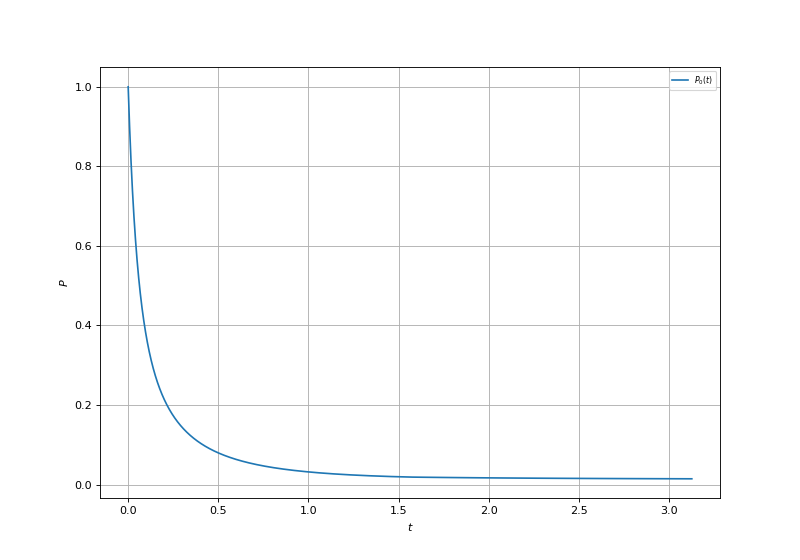
\includegraphics[width=\textwidth]{Images/P_o.png}}
\caption{Функция вероятности для 0 состояния}
\label{P_o}
\end{figure}

\begin{figure}[H]
\centerline{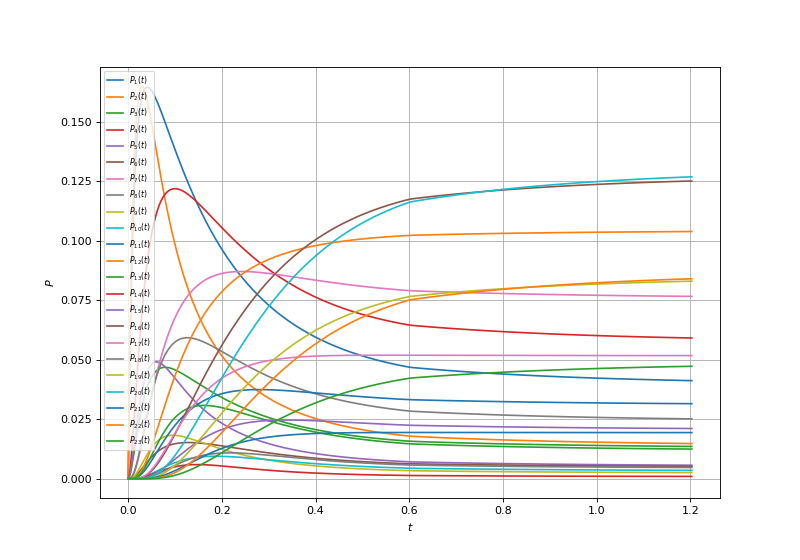
\includegraphics[width=\textwidth]{Images/P_i.png}}
\caption{Функции вероятностей для всех состояний (помимо 0) }
\label{P_i}
\end{figure}

\subsubsection{Прикладные характеристики системы}

Функция отказа может быть определена следующим образом:
$$1-R(t) = P_{term}(t)$$

График функции отказа $1-R(t)$ представлен на рисунке \ref{R_t}.
\begin{figure}[H]
\centerline{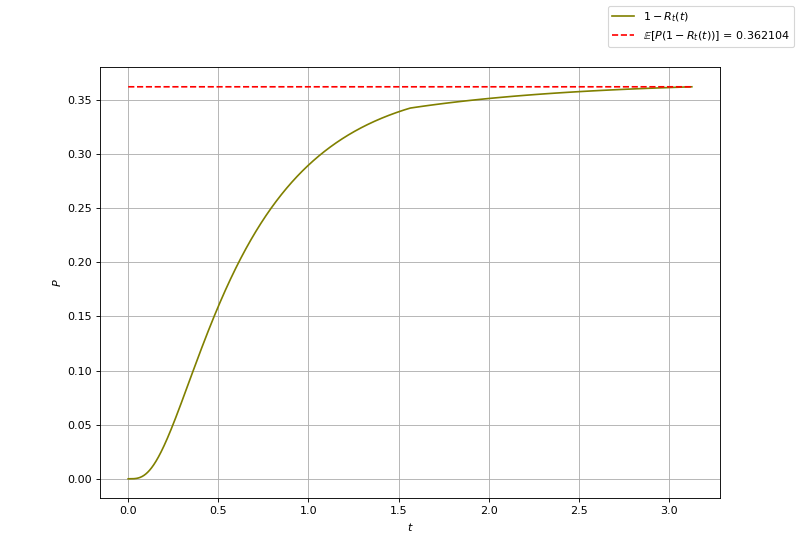
\includegraphics[width=\textwidth]{Images/R_t.png}}
\caption{Функция отказа системы}
\label{R_t}
\end{figure}

\begin{itemize}
    \item Математическое ожидание вероятности отказа:
$\mathbb{E}[P(1-R_t(t))]=0.362104 $;
\item Коэффициент загрузки ремонтной службы: $0.99615$;
\item Среднее число готовых к эксплуатации устройств типа  A и B: $1.5, 5.0$ соответственно;
\end{itemize}

\subsubsection{Имитационное моделирование системы}

Для системы с непрерывным временем была реализована функция, осуществляющая переходы по состояниям.

\begin{lstlisting}[language=python, label=prog,caption={\textit{реализация марковского процесса}}]
# моделирование одного эпизода с непрерывным временем
def MD(m):
    current_s = 0
    current_t = 0
    states_tr = [current_s]
    t_tr = [0]
    times = np.zeros(len(m))
    last = np.zeros(len(m))

    while 1:
        l_b, l_a, l_s = find_lambda(m[current_s])
         # -log(1-y)/(lambda_a+lambda_b)
        t_cur_s = F_t(l_a[0] + l_b[0] + l_s[0],
                      np.random.uniform(low=0.0, high=1.0, size=None))

        times[current_s] += t_cur_s
        current_t += t_cur_s
        idx_b = l_b[1]
        idx_a = l_a[1]
        idx_s = l_s[1]
        current_s = np.random.choice([idx_a, idx_b, idx_s],
                                     p=[l_a[0] / (l_a[0] + l_b[0] + l_s[0]),
                                        l_b[0] / (l_a[0] + l_b[0] + l_s[0]),
                                        l_s[0] / (l_a[0] + l_b[0] + l_s[0])])
        # для дальнейшей отрисовки
        states_tr.append(current_s)
        t_tr.append(current_t)

        if distance.euclidean(times / current_t, last)<0.00001:
            return states_tr, t_tr, [np.mean(w_A), np.mean(w_B)], times / current_t, current_t

        last = times / current_t
\end{lstlisting}



На рисунке \ref{MDP} представлен график переключению состояний системы для 1 прогона ($N=1$).
\begin{figure}[H]
\centerline{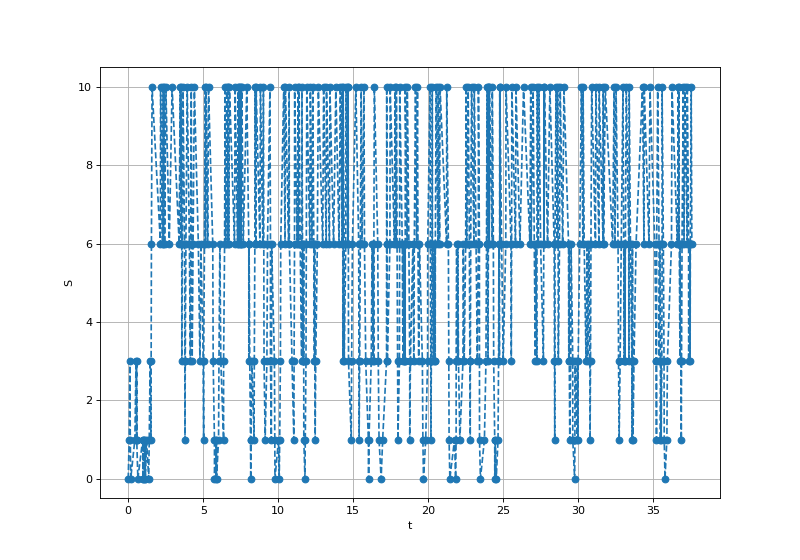
\includegraphics[width=\textwidth]{Images/term.png}}
\caption{График переключению состояний системы}
\label{MDP}
\end{figure}

Для $N=100$:
\begin{itemize}
    \item Среднее $t$ выхода на установившийся режим работы $24.113639752443333$;

    \item Статистические оценки предельных вероятностей после выхода на установившийся режим:
    \[
    \resizebox{\textwidth}{!}{$
[0.07, 0.11, 0.0, 0.17, 0.0, 0.0, 0.26, 0.0, 0.0, 0.0, 0.39, 0.0, 0.0, 0.0, 0.0, 0.0, 0.0, 0.0, 0.0, 0.0, 0.0, 0.0, 0.0, 0.0]
     $}
\]

\end{itemize}

\subsection{Дискретно-событийное моделирование системы}

Основные элементы дискретно-событийного моделирования системы:
\begin{itemize}
    \item Часы -- текущее "время" внутри моделирования.
    \item События -- поломка или починка устройства.
\end{itemize}
Блок-схема алгортима дискретно-событийного моделирования представлена на рисунке \ref{BS}

\begin{figure}[H]
\centerline{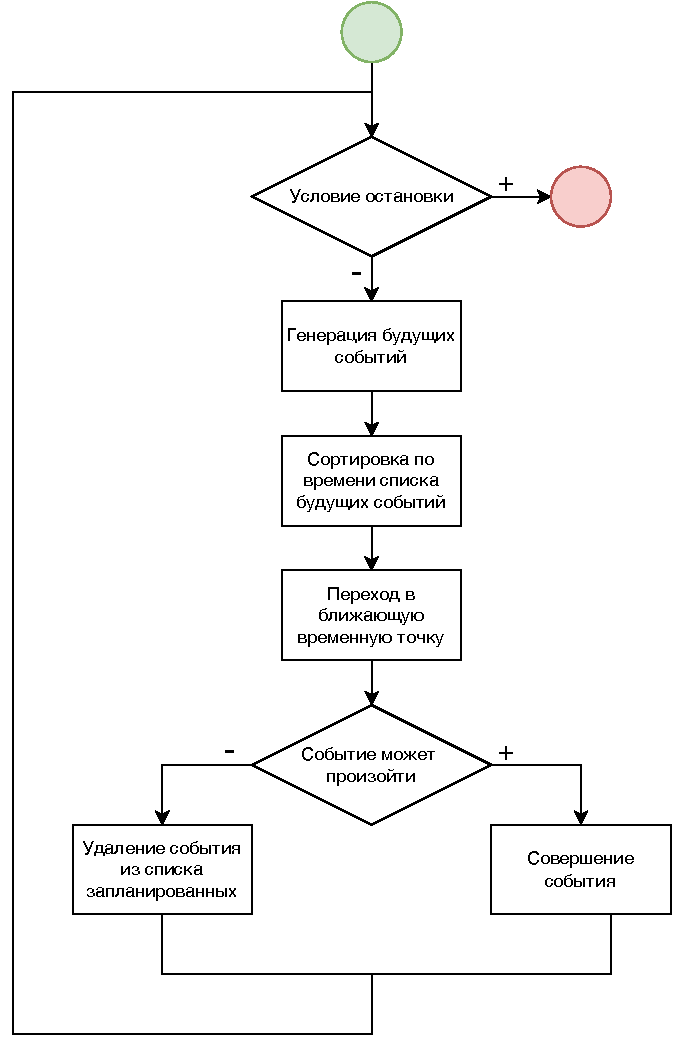
\includegraphics[width=0.5\textwidth]{Images/BS.pdf}}
\caption{Блок-схема алгоритма дискретно-событийного моделирования}
\label{BS}
\end{figure}

Результаты моделирования при $N=1$:
\scriptsize
\begin{verbatim}
Сломан A в момент времени 0.171 всего устройств типа А и В 4 5
                                                  --------------> 3 5
Починен A в момент времени 0.222 всего устройств типа А и В 3 5
                                                  --------------> 4 5
Сломан A в момент времени 0.244 всего устройств типа А и В 4 5
                                                  --------------> 3 5
Сломан B в момент времени 0.369 всего устройств типа А и В 3 5
                                                  --------------> 3 4
Сломан A в момент времени 0.402 всего устройств типа А и В 3 4
                                                  --------------> 2 4
Сломан A в момент времени 0.406 всего устройств типа А и В 2 4
                                                  --------------> 1 4
Починен A в момент времени 0.432 всего устройств типа А и В 1 4
                                                  --------------> 2 4
Сломан B в момент времени 0.446 всего устройств типа А и В 2 4
                                                  --------------> 2 3
Сломан A в момент времени 0.492 всего устройств типа А и В 2 3
                                                  --------------> 1 3
Сломан B в момент времени 0.497 всего устройств типа А и В 1 3
                                                  --------------> 1 2
Сломан A в момент времени 0.648 всего устройств типа А и В 1 2
                                                  --------------> пропуск события ввиду неработоспособности системы
Починен A в момент времени 0.795 всего устройств типа А и В 1 2
                                                  --------------> 2 2
Починен A в момент времени 0.804 всего устройств типа А и В 2 2
                                                  --------------> 3 2
Сломан A в момент времени 0.809 всего устройств типа А и В 3 2
                                                  --------------> 2 2
Сломан B в момент времени 0.860 всего устройств типа А и В 2 2
                                                  --------------> пропуск события ввиду неработоспособности системы
Починен B в момент времени 1.019 всего устройств типа А и В 2 2
                                                  --------------> 2 3
Починен A в момент времени 1.104 всего устройств типа А и В 2 3
                                                  --------------> 3 3
Сломан B в момент времени 1.114 всего устройств типа А и В 3 3
                                                  --------------> 3 2
Сломан B в момент времени 1.125 всего устройств типа А и В 3 2
                                                  --------------> пропуск события ввиду неработоспособности системы
Сломан A в момент времени 1.197 всего устройств типа А и В 3 2
                                                  --------------> 2 2
Сломан B в момент времени 1.257 всего устройств типа А и В 2 2
                                                  --------------> пропуск события ввиду неработоспособности системы
Сломан A в момент времени 1.418 всего устройств типа А и В 2 2
                                                  --------------> 1 2
Сломан A в момент времени 1.426 всего устройств типа А и В 1 2
                                                  --------------> пропуск события ввиду неработоспособности системы
Сломан B в момент времени 1.446 всего устройств типа А и В 1 2
                                                  --------------> пропуск события ввиду неработоспособности системы
Сломан A в момент времени 1.486 всего устройств типа А и В 1 2
                                                  --------------> пропуск события ввиду неработоспособности системы
Починен A в момент времени 1.510 всего устройств типа А и В 1 2
                                                  --------------> 2 2
Сломан A в момент времени 1.526 всего устройств типа А и В 2 2
                                                  --------------> 1 2
Починен A в момент времени 1.828 всего устройств типа А и В 1 2
                                                  --------------> 2 2
Сломан B в момент времени 1.829 всего устройств типа А и В 2 2
                                                  --------------> пропуск события ввиду неработоспособности системы
Починен A в момент времени 1.977 всего устройств типа А и В 2 2
                                                  --------------> 3 2
Починен B в момент времени 1.991 всего устройств типа А и В 3 2
                                                  --------------> 3 3
Починен A в момент времени 2.005 всего устройств типа А и В 3 3
                                                  --------------> 4 3
Починен A в момент времени 2.035 всего устройств типа А и В 4 3
                                                  --------------> пропуск события ввиду исправности всех устройств типа А
Починен A в момент времени 2.254 всего устройств типа А и В 4 3
                                                  --------------> пропуск события ввиду исправности всех устройств типа А
Сломан B в момент времени 2.297 всего устройств типа А и В 4 3
                                                  --------------> 4 2
Сломан B в момент времени 2.320 всего устройств типа А и В 4 2
                                                  --------------> пропуск события ввиду неработоспособности системы
Сломан B в момент времени 2.373 всего устройств типа А и В 4 2
                                                  --------------> пропуск события ввиду неработоспособности системы
Починен A в момент времени 2.561 всего устройств типа А и В 4 2
                                                  --------------> пропуск события ввиду исправности всех устройств типа А
Сломан A в момент времени 2.651 всего устройств типа А и В 4 2
                                                  --------------> 3 2
Починен A в момент времени 2.685 всего устройств типа А и В 3 2
                                                  --------------> 4 2
Сломан A в момент времени 2.703 всего устройств типа А и В 4 2
                                                  --------------> 3 2
Починен B в момент времени 2.709 всего устройств типа А и В 3 2
                                                  --------------> 3 3
Починен A в момент времени 2.743 всего устройств типа А и В 3 3
                                                  --------------> 4 3
Сломан A в момент времени 2.746 всего устройств типа А и В 4 3
                                                  --------------> 3 3
Починен B в момент времени 2.770 всего устройств типа А и В 3 3
                                                  --------------> 3 4
Починен A в момент времени 2.778 всего устройств типа А и В 3 4
                                                  --------------> 4 4
Починен B в момент времени 2.817 всего устройств типа А и В 4 4
                                                  --------------> 4 5
Починен A в момент времени 2.818 всего устройств типа А и В 4 5
                                                  --------------> пропуск события ввиду исправности всех устройств типа А
Починен A в момент времени 2.850 всего устройств типа А и В 4 5
                                                  --------------> пропуск события ввиду исправности всех устройств типа А
Сломан A в момент времени 2.928 всего устройств типа А и В 4 5
                                                  --------------> 3 5
Сломан B в момент времени 2.994 всего устройств типа А и В 3 5
                                                  --------------> 3 4
Починен A в момент времени 3.206 всего устройств типа А и В 3 4
                                                  --------------> 4 4
Починен A в момент времени 3.215 всего устройств типа А и В 4 4
                                                  --------------> пропуск события ввиду исправности всех устройств типа А
Починен B в момент времени 3.216 всего устройств типа А и В 4 4
                                                  --------------> 4 5
Починен A в момент времени 3.216 всего устройств типа А и В 4 5
                                                  --------------> пропуск события ввиду исправности всех устройств типа А
Починен A в момент времени 3.256 всего устройств типа А и В 4 5
                                                  --------------> пропуск события ввиду исправности всех устройств типа А
Починен B в момент времени 3.289 всего устройств типа А и В 4 5
                                                  --------------> пропуск события ввиду исправности всех устройств типа В
Починен A в момент времени 3.322 всего устройств типа А и В 4 5
                                                  --------------> пропуск события ввиду исправности всех устройств типа А
Сломан A в момент времени 3.335 всего устройств типа А и В 4 5
                                                  --------------> 3 5
Сломан B в момент времени 3.390 всего устройств типа А и В 3 5
                                                  --------------> 3 4
Сломан B в момент времени 3.469 всего устройств типа А и В 3 4
                                                  --------------> 3 3
Сломан B в момент времени 3.587 всего устройств типа А и В 3 3
                                                  --------------> 3 2
Починен B в момент времени 3.688 всего устройств типа А и В 3 2
                                                  --------------> 3 3
Сломан B в момент времени 3.698 всего устройств типа А и В 3 3
                                                  --------------> 3 2
Починен B в момент времени 3.755 всего устройств типа А и В 3 2
                                                  --------------> 3 3
Починен A в момент времени 3.771 всего устройств типа А и В 3 3
                                                  --------------> 4 3
Починен A в момент времени 3.838 всего устройств типа А и В 4 3
                                                  --------------> пропуск события ввиду исправности всех устройств типа А
Сломан B в момент времени 3.871 всего устройств типа А и В 4 3
                                                  --------------> 4 2
Починен A в момент времени 3.874 всего устройств типа А и В 4 2
                                                  --------------> пропуск события ввиду исправности всех устройств типа А
Починен A в момент времени 3.923 всего устройств типа А и В 4 2
                                                  --------------> пропуск события ввиду исправности всех устройств типа А
Сломан A в момент времени 3.973 всего устройств типа А и В 4 2
                                                  --------------> 3 2
Починен A в момент времени 3.978 всего устройств типа А и В 3 2
                                                  --------------> 4 2
Починен B в момент времени 4.011 всего устройств типа А и В 4 2
                                                  --------------> 4 3
Сломан A в момент времени 4.329 всего устройств типа А и В 4 3
                                                  --------------> 3 3
Починен A в момент времени 4.338 всего устройств типа А и В 3 3
                                                  --------------> 4 3
Починен A в момент времени 4.352 всего устройств типа А и В 4 3
                                                  --------------> пропуск события ввиду исправности всех устройств типа А
Починен A в момент времени 4.353 всего устройств типа А и В 4 3
                                                  --------------> пропуск события ввиду исправности всех устройств типа А
Сломан B в момент времени 4.378 всего устройств типа А и В 4 3
                                                  --------------> 4 2
Починен B в момент времени 4.380 всего устройств типа А и В 4 2
                                                  --------------> 4 3
Починен A в момент времени 4.393 всего устройств типа А и В 4 3
                                                  --------------> пропуск события ввиду исправности всех устройств типа А
Починен A в момент времени 4.416 всего устройств типа А и В 4 3
                                                  --------------> пропуск события ввиду исправности всех устройств типа А
Починен B в момент времени 4.437 всего устройств типа А и В 4 3
                                                  --------------> 4 4
Починен B в момент времени 4.473 всего устройств типа А и В 4 4
                                                  --------------> 4 5
Сломан B в момент времени 4.902 всего устройств типа А и В 4 5
                                                  --------------> 4 4
Сломан A в момент времени 5.124 всего устройств типа А и В 4 4
                                                  --------------> 3 4
Починен B в момент времени 5.134 всего устройств типа А и В 3 4
                                                  --------------> 3 5
Сломан A в момент времени 5.143 всего устройств типа А и В 3 5
                                                  --------------> 2 5
Сломан B в момент времени 5.153 всего устройств типа А и В 2 5
                                                  --------------> 2 4
Починен A в момент времени 5.161 всего устройств типа А и В 2 4
                                                  --------------> 3 4
Починен B в момент времени 5.183 всего устройств типа А и В 3 4
                                                  --------------> 3 5
Починен B в момент времени 5.201 всего устройств типа А и В 3 5
                                                  --------------> пропуск события ввиду исправности всех устройств типа В
Починен A в момент времени 5.209 всего устройств типа А и В 3 5
                                                  --------------> 4 5
Сломан B в момент времени 5.213 всего устройств типа А и В 4 5
                                                  --------------> 4 4
Починен A в момент времени 5.268 всего устройств типа А и В 4 4
                                                  --------------> пропуск события ввиду исправности всех устройств типа А
Починен A в момент времени 5.386 всего устройств типа А и В 4 4
                                                  --------------> пропуск события ввиду исправности всех устройств типа А
Починен A в момент времени 5.394 всего устройств типа А и В 4 4
                                                  --------------> пропуск события ввиду исправности всех устройств типа А
Починен B в момент времени 5.969 всего устройств типа А и В 4 4
                                                  --------------> 4 5
Починен B в момент времени 5.987 всего устройств типа А и В 4 5
                                                  --------------> пропуск события ввиду исправности всех устройств типа В
Сломан A в момент времени 5.997 всего устройств типа А и В 4 5
                                                  --------------> 3 5
Сломан B в момент времени 6.002 всего устройств типа А и В 3 5
                                                  --------------> 3 4
Починен A в момент времени 6.008 всего устройств типа А и В 3 4
                                                  --------------> 4 4
Починен A в момент времени 6.031 всего устройств типа А и В 4 4
                                                  --------------> пропуск события ввиду исправности всех устройств типа А
Починен A в момент времени 6.040 всего устройств типа А и В 4 4
                                                  --------------> пропуск события ввиду исправности всех устройств типа А
Починен B в момент времени 6.044 всего устройств типа А и В 4 4
                                                  --------------> 4 5
Сломан A в момент времени 6.128 всего устройств типа А и В 4 5
                                                  --------------> 3 5
Починен A в момент времени 6.130 всего устройств типа А и В 3 5
                                                  --------------> 4 5
Починен A в момент времени 6.134 всего устройств типа А и В 4 5
                                                  --------------> пропуск события ввиду исправности всех устройств типа А
Сломан B в момент времени 6.507 всего устройств типа А и В 4 5
                                                  --------------> 4 4
Починен A в момент времени 6.737 всего устройств типа А и В 4 4
                                                  --------------> пропуск события ввиду исправности всех устройств типа А
Починен B в момент времени 6.740 всего устройств типа А и В 4 4
                                                  --------------> 4 5
Починен B в момент времени 6.782 всего устройств типа А и В 4 5
                                                  --------------> пропуск события ввиду исправности всех устройств типа В
Починен A в момент времени 6.789 всего устройств типа А и В 4 5
                                                  --------------> пропуск события ввиду исправности всех устройств типа А
Починен B в момент времени 6.812 всего устройств типа А и В 4 5
                                                  --------------> пропуск события ввиду исправности всех устройств типа В
Починен A в момент времени 6.837 всего устройств типа А и В 4 5
                                                  --------------> пропуск события ввиду исправности всех устройств типа А
Сломан A в момент времени 6.975 всего устройств типа А и В 4 5
                                                  --------------> 3 5
Починен A в момент времени 6.986 всего устройств типа А и В 3 5
                                                  --------------> 4 5
Починен A в момент времени 7.132 всего устройств типа А и В 4 5
                                                  --------------> пропуск события ввиду исправности всех устройств типа А
Сломан B в момент времени 7.151 всего устройств типа А и В 4 5
                                                  --------------> 4 4

\end{verbatim}
\normalsize

Статистические данные при $N=100$:
\begin{itemize}
    \item Cреднее число готовых к эксплуатации устройств типа A и B = $ 3.29, 3.94 $,
    \item Среднее время выхода в установившийся режим работы = $ 4.407275403114299 $
\end{itemize}
%-------------------------------------------------
\subsection{Вывод}
В ходе выполнения домашнего задания была промоделирована работа СМО в терминах непрерывных марковских цепей,
а также выполнен анализ ее работы.

% --------------------------------------
% Атрибуты задачи
\labattributes{}{}{}{}{студент группы \EduGroup, \Author}{\Year, \Semestr}
%--------------
